%%%%%%%%%%%%%%%%%%%%%%%%%%%%%%%%%%%%%%%%%%%%%%%%%%%%%%%
% ultimate plantUML Cheatsheet
%   by Andreas Offenhaeuser
% Based on MatPlotLib Cheatsheet by Michelle Baltazar https://www.overleaf.com/latex/examples/matplotlib-and-random-cheat-sheet/yttxrcxntbht
%
%%%%%%%%%%%%%%%%%%%%%%%%%%%%%%%%%%%%%%%%%%%%%%%%%%%%%%%

\documentclass{article}
\usepackage[landscape]{geometry}
\usepackage[T1]{fontenc}
\usepackage{multicol}
\usepackage{scrextend}
\usepackage{amsfonts}
\usepackage[most]{tcolorbox}
\usepackage{tikz}
\usetikzlibrary{decorations.pathmorphing}
\usepackage{xcolor}

\definecolor{white}{RGB}{255,255,255}
\definecolor{darkgray}{HTML}{333333}
\definecolor{gray}{HTML}{4D4D4D}

\usepackage{hyperref}
\hypersetup{
    colorlinks, breaklinks,
    linkcolor={red!50!black},
    citecolor={blue!50!black},
    urlcolor={blue!80!black}
}
\advance\topmargin-.8in
\advance\textheight3in
\advance\textwidth3in
\advance\oddsidemargin-1.5in
\advance\evensidemargin-1.5in
\parindent0pt
\parskip2pt

\newcommand{\block}[2]{%
  \begin{tikzpicture}%
  \node [draw=black, fill=white, very thick,
rectangle, rounded corners, inner sep=10pt, inner ysep=10pt] (box){%
    \begin{minipage}{0.3\textwidth}%
		#2%
    \end{minipage}%
  };%
\node[fill=black, text=white, font=\bfseries, right=10pt] at (box.north west) {#1};
\end{tikzpicture}%
}

\newcommand{\code}[1]{%
  \begin{tcolorbox}[frame hidden, interior hidden, grow to left by=-5pt,
  boxrule=0pt, boxsep=0pt, arc=0pt, breakable, before skip=4pt, after skip=5pt,]%
  #1%
  \end{tcolorbox}
}

\title{ultimate plantUML Cheatsheet}
\begin{document}

\begin{center}{\huge{\textbf{ultimate plantUML Cheatsheet}}}\\
{\large by \href{http://anoff.io}{Andreas Offenhaeuser}}
\end{center}
\begin{multicols*}{3}


\block{Components}{
A list of plantUML components and their names, most can be used in any diagrams. The \textit{sequence} diagram only supports a subset.
  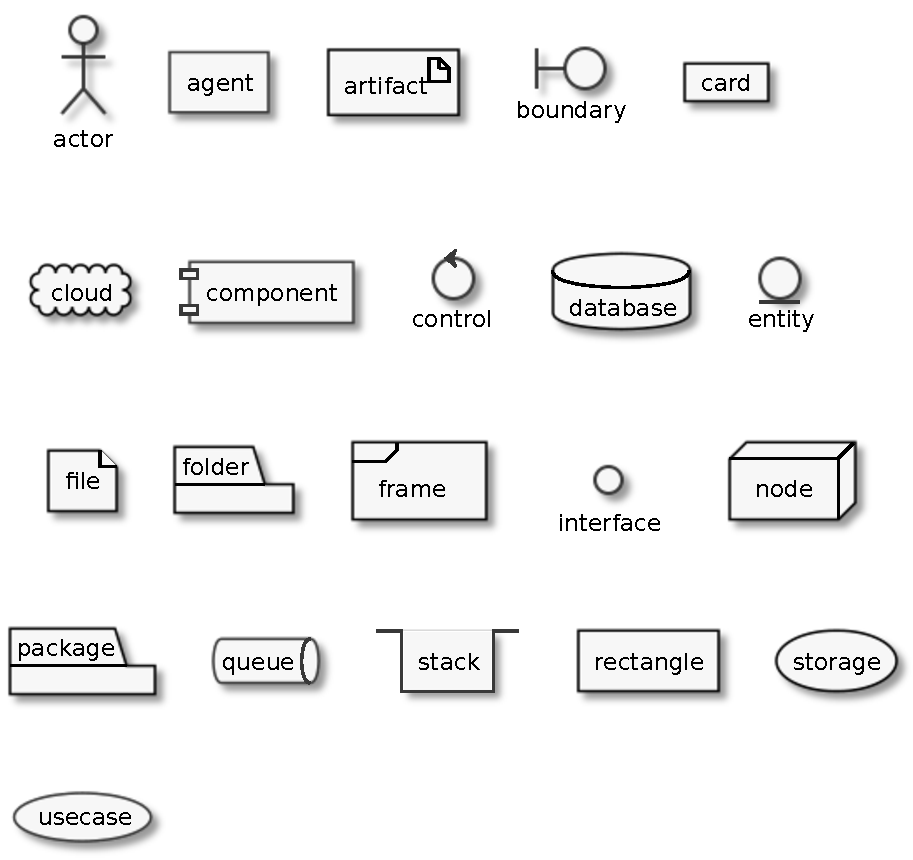
\includegraphics[width=\textwidth]{diagrams/dist/components.pdf} 
}

\block{Icons}{
PlantUML supports \href{https://useiconic.com/open/}{Open Iconic} iconset out of the box. Any icon can be rendered when embedding it in \textbf{<\&..>}
\code{
card "<\&key> key"

card "<size:42><\&wrench></size>"
}
  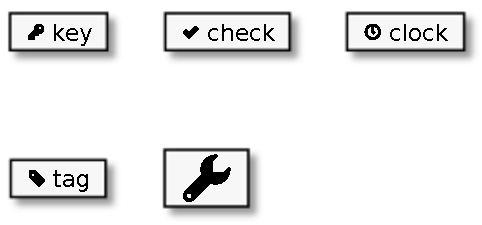
\includegraphics[width=0.7\textwidth]{diagrams/dist/icons.pdf} 
}

\block{Multiline components}{
Text can be spread across multiple lines in components by declaring the text in \textbf{[ ]}
\code{
node mynode [
\begin{addmargin}[1em]{0em}
    several \\
    lines \\
    ==== \\
    of \\
    .... \\
    text
\end{addmargin}
]
}
  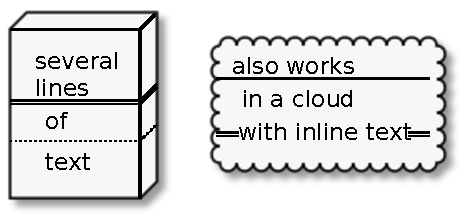
\includegraphics[width=0.7\textwidth]{diagrams/dist/multiline.pdf} 
}

\block{Useful links}{
  \begin{itemize}
  \item \href{http://plantuml.com/color}{Available colors}
  \item \href{http://plantuml.com/skinparam}{Stylable properties}
\end{itemize}
}
\end{multicols*}
\end{document}